%%% This Beamer example was created by LianTze Lim, April 2017.

%%%% This is a VERY simple and minimalistic beamer theme,
%%%% even reminiscent of marker pens on transparencies!
%%%% It mimics the look of the "seminar" package, which
%%%% can only be used with plain TeX.
%%%% There are also some comments and example to show how
%%%% to customise various elements, e.g. the font and colours.

\documentclass[12pt]{beamer}
%% If you'd like the default font size to be even larger, use 14pt or 17pt; these are supported by Beamer.

\graphicspath{{Figures/}{Figures}}

%%%%%%%%%%%%%%%%%%%%%%%%%%%%%%%%%%%%%%%%%
% These lines should usually go into a .sty file,
% but I'll leave them here so that it's easier to
% see how to customise a Beamer theme.
% Remember, the Beamer manual is your friend!!
% http://texdoc.net/pkg/beamer
%
%% So if your re-definitions have a @ somewhere, you
%% _MUST_ put a \makeatletter before these lines and then
%% \makeatother after them. This trick can only be done
%% in the preamble! BUT if you're doing these re-definitions
%% in a .sty file (so that you \usepackage it later), you
%% don't need the \makeatletter and \makeatother.
\makeatletter

%% Set the left and right margins
\setbeamersize{text margin left=1em,text margin right=1em}

%% FONTS
\setbeamerfont{title}{series=\bfseries,size=\LARGE}
\setbeamerfont{subtitle}{series=\bfseries,size=\Large}
\setbeamerfont{frametitle}{series=\bfseries,size=\small}
\setbeamerfont{block title}{series=\bfseries,size=\normalsize}
\setbeamerfont{footline}{size=\small}

%% COLOURS
%% If you'd like everything to have the same colour
\usebeamercolor{structure}
\setbeamercolor{normal text}{fg=structure.fg}

%% Add a line after the frametitle
\addtobeamertemplate{frametitle}{}{\vspace*{-1ex}\rule{\textwidth}{1pt}}

%% Use circular discs as itemized list markers;
%% there's an existing option in Beamer for it so I'll use it
\setbeamertemplate{itemize items}[circle]

%% Remove default navigation symbols (We'll add the ones we need in the footline
\setbeamertemplate{navigation symbols}{}


%% And before the footline... actually we'd like to re-define
%% the footline
\setbeamertemplate{footline}{%
   %% Beamer headlines and footlines are always full-paperwidth, so if you want the horizontal line to
   %% not span it entirely you'll need to do a bit of arithmetic
   \centering
   \begin{minipage}{\dimexpr\paperwidth-\beamer@leftmargin-\beamer@rightmargin\relax}
   \centering
   \rule{\linewidth}{1pt}\vskip2pt
   \usebeamerfont{footline}%
   \usebeamercolor{footline}%
   %% The frame number smack in the middle
   \hfill\insertframenumber/\inserttotalframenumber
   \hfill%
   %% ONLY the navigation symbols we want at the far right.
   %% We use an \llap so that it takes up zero width, and doesn't throw the page number off-centre!
   \llap{\insertframenavigationsymbol\insertbackfindforwardnavigationsymbol}\par
   \end{minipage}\vskip2pt
}

\setbeamercolor{block title alerted}{fg=white,bg=brown}

\makeatother
%%%% END STYLE CUSTOMISATION %%%%%%%%%%%%

\usepackage[english]{babel}

\usepackage{graphicx}

\usepackage[latin1]{inputenc}
\usepackage[T1]{fontenc}

\usepackage{subcaption}

\usepackage{times}

\usepackage{graphics}
%\usepackage[draft]{graphics}

\usepackage{xspace}
\usepackage{amsmath}
\usepackage{bm}
\usepackage{pgfpages}
\usepackage{fancybox}
\usepackage{threeparttable}
\usepackage{bbding}
\usepackage{verbatim}
\usepackage{booktabs}

\usepackage{natbib}
\bibpunct{(}{)}{;}{a}{}{,}

\newcommand{\pkg}[1]{{\normalfont\fontseries{b}\selectfont #1}}
\let\proglang=\textsf
\let\code=\texttt

\newcommand{\btheta}{ \mbox{\boldmath $\theta$}}
\newcommand{\bbeta}{ \mbox{\boldmath $\beta$}}
\newcommand{\balpha}{ \mbox{\boldmath $\alpha$}}
\newcommand{\by}{ \mbox{\bf y}}
\newcommand{\bY}{ \mbox{\bf Y}}
\newcommand{\bX}{ \mbox{\bf X}}
\newcommand{\bH}{ \mbox{\bf H}}
\newcommand{\bI}{ \mbox{\bf I}}


\title{Week 6 wrap-up}
\subtitle{}
\author{Bayesian modelling for spatial and spatio-temporal data}
\institute{MSc in Epidemiology}
\date{Week 6}


\begin{document}

\begin{frame}[t]
  \titlepage
\end{frame}

\begin{frame}
\begin{itemize} \setlength\itemsep{\fill}
\item This week we introduced the field of spatial analysis, which is based on the non-independence of the observations.
\item We can use spatial analysis to solve a number of problems, when the data are characterized by geographical attributes.
\item We started by classifying data into one of three basic types (based on the domain $\mathcal{D}$): 
\begin{itemize}
\item areal data, 
\item point-referenced (or geostatistical) data, 
\item random point pattern data.
%\item We saw also the fundamental spatial data types treated within the R environment: vector (mainly point, lines or polygons) and raster data.
\end{itemize}
\end{itemize}
\end{frame}

\begin{frame}
\frametitle{Type of spatial data}
\vspace{-10pt}
\begin{figure}
\begin{subfigure}{.4\textwidth}
\vspace{5pt}
  \centering
  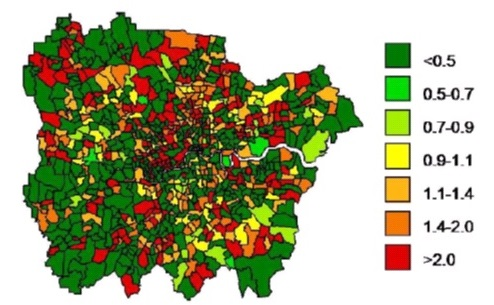
\includegraphics[width=.7\linewidth]{leukemia_1985_96.jpg}
  \caption{\tiny{\textbf{Areal data}\\  Map of SMR of leukaemia in children 0-15 yrs, 1985-96 for 872 wards in Greater London (Source: Best et al, 1991)}}
  %A spatial process is observed on a regular or irregular grid. Most of the time this arises due to aggregation of some sort}}
\end{subfigure}
\begin{subfigure}{.4\textwidth}
  \centering
  \vspace{9pt}
  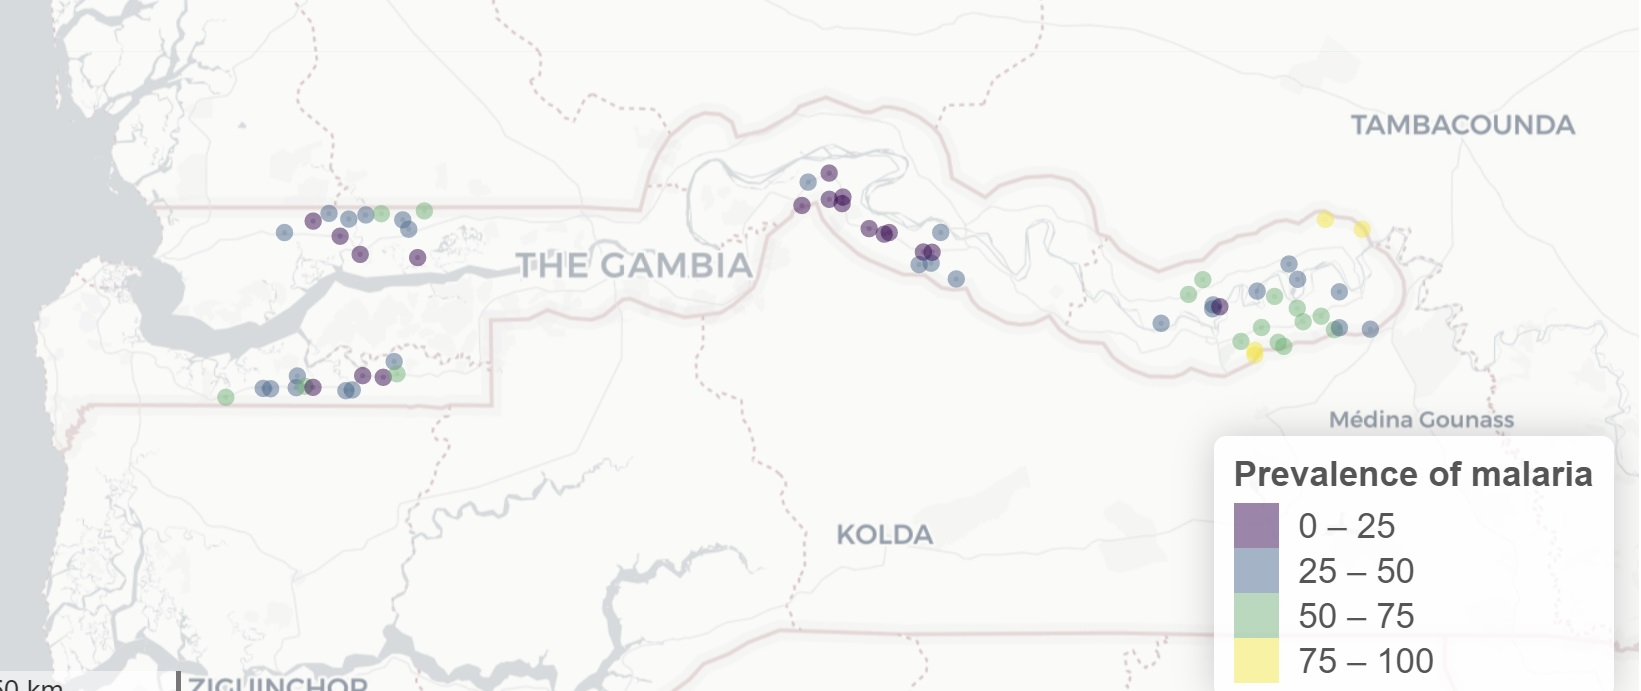
\includegraphics[width=.8\linewidth]{malaria_map2.jpg}
    \vspace{8pt}
  \hspace{15pt}\caption{\tiny{\textbf{Geostatistical data} \\  Prevalence of malaria among a sample of village
resident children in the Gambia (65 villages) (Source: Diggle et al, 2002)}}
  %A spatial process that varies continuously is observed only at a few points}}
\end{subfigure}
\begin{subfigure}{.5\textwidth}
  \centering
  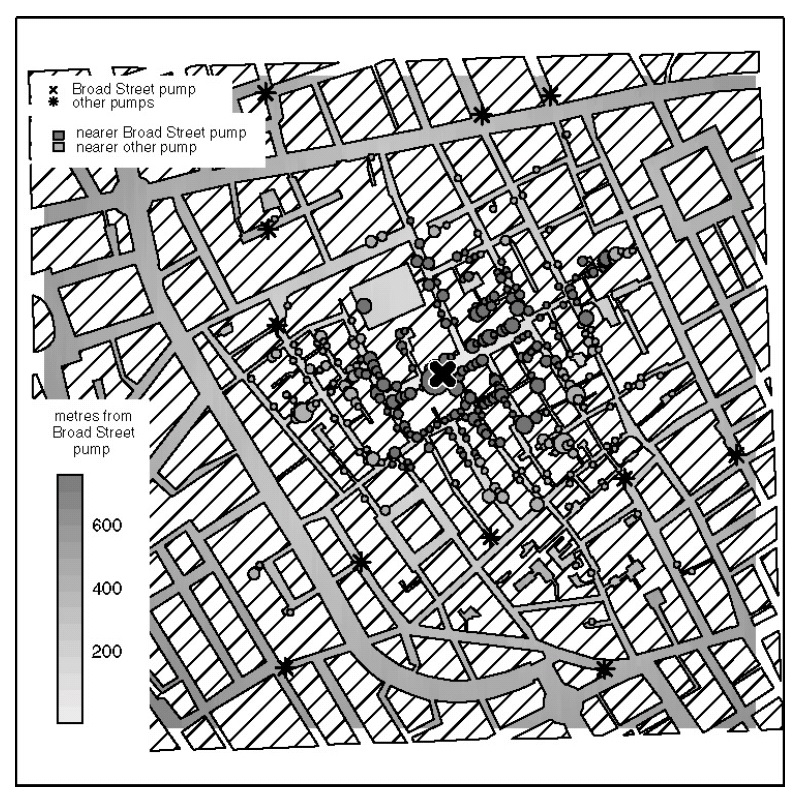
\includegraphics[width=.5\linewidth]{colera_pump.jpg}
  \caption{\tiny{\textbf{Point pattern data}\\ The 1854 London cholera outbreak near Golden Square in London (source: Bivand et al, Applied Spatial Data Analysis with R, Springer, 2013)}} %A spatial process is observed at a set of locations and the locations themselves are of interest}}
\end{subfigure}
%\label{fig:typeSpat}
\end{figure}
\end{frame}


\begin{frame}
\frametitle{Coordinate Reference System (CRS)}
\begin{itemize} \setlength\itemsep{\fill}
\item We introduced the concept of Coordinate Reference System (CRS), which defines how the spatial elements of the data relate to the surface of the Earth.
\item We introduced the difference between \alert{Geographic coordinate systems (GCS)} and \alert{Projected coordinate systems (PCS)}:
\begin{itemize}
  \item The GCS identify any location on the Earth's surface using longitude and
latitude, with units in decimal degrees or degrees.
  \item The PCS provide mechanisms to project maps of the Earth's ellipsoid shape onto a two-dimensional Cartesian coordinate plan.
\end{itemize}
\item Because the projections are a way to convert the Globe's curved surface into a two-dimensional plane, we introduce distorsion.
\end{itemize}
\end{frame}

\begin{frame}
\frametitle{Spatial autocorrelation}
\begin{itemize} \setlength\itemsep{\fill}
\item We focused on the key geographic concept of \alert{spatial autocorrelation}, which implies that observations from units closer to each other are more similar than those recorded in units farther away.
\item It quantifies the degree of which observations, at spatial locations, are similar to nearby observations.
\item  The detection of spatial autocorrelation is useful in spatial analysis for identifying underlying data structures, the degree of spatial randomness, or clustering in the data.
\item We saw how to construct \alert{spatial proximity weights}, that is weights that depend on the underline geography of the region.
%\item The spatial relationship between the areas can be represented as an adjacency matrix $\mathbf{W}$ with dimensions $N \times N$, where the entries $w_{ij}$ of the matrix are the spatial weights:
%\end{itemize}
%\begin{equation*}
%\mathbf{W} =
%\begin{bmatrix}
%w_{11} & w_{12} & \cdots & w_{1N} \\
%w_{21} & w_{22} & \cdots & w_{2N} \\
%\vdots  & \vdots  & \ddots & \vdots \\
%w_{N1} & w_{N2} & \cdots & w_{NN}
%\end{bmatrix}
%\end{equation*}
\end{itemize}
\end{frame}


\begin{frame}
\frametitle{How we define spatial neighbours?}
\begin{itemize} \setlength\itemsep{\fill}
\item \small{There are different ways to build the weights, according to the spatial neighborhood definition. We can define as neighbors areas that are  adjacent according to \textcolor{cyan}{rook} criterion (A), or \textcolor{cyan}{queen} criterion (B):}
\begin{columns}
\column{0.5\textwidth}
\begin{figure}
  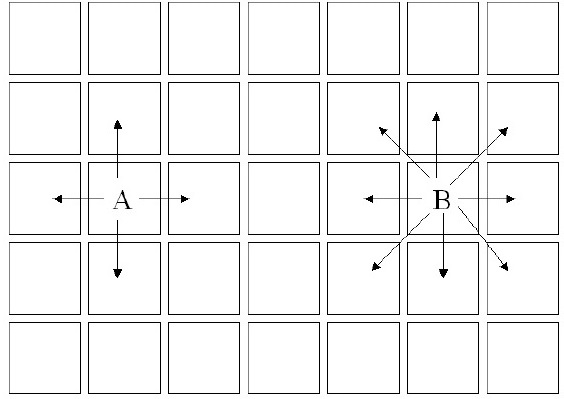
\includegraphics[width=1.5in]{Weights.jpg}
\end{figure}
\column{0.5\textwidth}
\small {In its simple form, $w_{ij}=1$ if areas $i$ and $j$ are adjacent, 0 otherwise.}
\end{columns}   
   
\item \small{We can expand the idea of neighborhood to include areas that are close, according to other definitions of proximity. Thus, we may take $w_{ij}=1$ for all $i$ and area $j$ within a specified distance, or for a given area $i$, we may take $w_{ij}=1$ if $j$ is one of the $k$ nearest neighbors of $i$.}
\end{itemize}
\end{frame}


\begin{frame}
\frametitle{Measuring spatial autocorrelation}
\begin{itemize}\setlength\itemsep{\fill}
\item A number of approaches have been suggested for measuring spatial autocorrelation.
\item Global measures of spatial autocorrelation share a common structure: calculate the similarity of values at locations $i$ and $j$, then weight the similarity by the proximity of locations $i$ and $j$.
\item Null hypothesis: spatial randomness. 
\item We saw an example of global measure given by the Moran's I test, that can be applied to the data directly, or to the residuals from a regression model.
%\item Let $\{Z_{i}: i,\dots,N\}$ represent spatially referenced data (or residuals) for $N$ spatial locations.
%\item The global Moran'I statistic is:\\
%\footnotesize{$$ I  = \frac{N \sum_{i=1}^N \sum_{j=1}^N w_{ij}(Z_i - \overline{Z})(Z_j - \overline{Z})}
%{\left(\sum_i\sum_j w_{ij}\right)\sum_{i=1}^N (Z_i - \overline{Z})^2} $$
%\vspace{5pt}
%where $\overline{Z}=(1/N)\sum_i^N Z_i$ is the spatial mean and $w_{ij}$ are the weights}
\end{itemize}
\end{frame}

\begin{frame}
\frametitle{Starting a disease mapping analysis}
\begin{itemize} \setlength\itemsep{\fill}
\item Collect (age and/or sex stratum-specific) morbidity or mortality data for each area $i$, $i=1,\dots, N$, and population data
\item Compute the expected cases (i.e. number of disease cases would be expected if the study population had
the stratum distribution of a reference population)  
\item Compute the SMR or SIR for each area $i$ as:
    \begin{equation*}
    SMR_i \hspace{2pt} \text{or} \hspace{2pt}  SIR_i = \frac{\text{Observed nb. cases in area } i}{\text{Expected nb. cases in area }   i}
    \end{equation*}
\begin{itemize}
\footnotesize{
\item $SMR_i = 1$: the area $i$ has equal number of observed and expected cases (equal $i$ has the same risk that the standard population)
\item $SMR_i <1$: the area $i$ has less observed cases than expected cases (area $i$ has lower risk than the standard population)
\item $SMR_i >1$: the area $i$ has more observed cases than expected cases (area $i$ has higher risk than the standard population)}
\end{itemize}
\end{itemize}
\end{frame}


\begin{frame}
\frametitle{Problem with mapping the SMRs or SIRs}
\small{
\begin{itemize} \setlength\itemsep{\fill}
  \item A map of raw SMRs or SIRs can be unstable or misleading, particularly if the estimates are based on populations of very different sizes. In fact, since the variability in the estimated local risks depends on population size, some risks may be better estimated than others, and this may obscure spatial patterns in disease risk.
%A map of raw risks, such as a map of SIRs, may obscure the spatial pattern in disease risk, Indeed, risks based on small numbers of disease cases or on small populations are likely to be elevated artificially, reflecting lack of data rather than true elevated risk.
\item For example, SMRs or SIRs based on small populations or on small numbers of disease cases (e.g. rare diseases) are very imprecise, as areas with small expected number of cases have high associated variance.
\item They ignore possible spatial correlation between disease risk in nearby areas, due to possible dependence on spatially varying risk factors. %Another problem in using conventional Poisson based methods is that they do not take account of any spatial pattern of disease, i.e. they ignore the fact that areas geographically close to one another share similar disease rates and common factors which influence the incidence and outcome of disease
\item They do not allow the inclusion of ecological covariates. %Inclusion of such variables would allow the construction of disease maps that take into account risk factors that are known to affect a specific disease.

\end{itemize}
}
\end{frame}


\begin{frame}
\frametitle{Smoothing}
\begin{itemize} \setlength\itemsep{\fill}
\item \alert{Smoothed} estimates of the RRs provide more robust estimates. 
\item The basic idea is to \alert{borrow information} from neighbouring areas to produce a better (i.e. more stable and less noisy) estimate of the risk associated with each area and thus separate out the signal from the noise.
\item This week we study a non-spatial smoothing of the estimates of RRs.
\end{itemize}
\end{frame}

\begin{frame}
    \frametitle{The Poisson log-Normal model (non-spatial smoothing)}
\vspace{-10pt}
\footnotesize{
\begin{eqnarray*}
O_i & \sim & \hbox{Poisson}(\lambda_i E_i) \\
%\mu_i=\lambda_i E_i \\
\log(\lambda_i) & = & \alpha + \theta_i\\
\theta_i & \sim  & \hbox{Normal}(0, \sigma_{\theta}^2) \\
\alpha &\sim & \hbox{Normal}(0,10^4)\\
1/\sigma^2_{\theta} &\sim &\text{Gamma}(1, 0.01)\\
\end{eqnarray*}
}
\vspace{-10pt}
{\footnotesize
\begin{itemize}\setlength\itemsep{\fill}
\item $O_i$ and $E_i$ are observed and expected number of cases in area $i$
\item $\lambda_i$ is the unknown area-specific relative risk of morbidity or mortality from the disease
 \item Parameter $\alpha$ is mean log relative risk, i.e. overall risk in the region of study
\item  Parameters $\theta_i$: {\bf area-specific random effects} to capture region-wide heterogeneity. They take into account the extra-Poisson variability, i.e.  \alert{overdispersion}, in the log-relative risks %The excess variation can be due to:
  %\begin{itemize} \setlength\itemsep{\fill}
  %  \item errors in numerators (observed counts) and denominators (expected counts)
   % \item unobserved or unknown risk factors (confounders)
 % \end{itemize}
 % \item  residual RR = $\exp (\theta_i)$
  \item $\sigma_{\theta}^2$: controls the magnitude of the $\theta_i$ %reflects the amount of extra-Poisson variation in the data
\end{itemize}
}
\end{frame}


\begin{frame}
\frametitle{Disease mapping in action: our labs}
\begin{itemize} \setlength\itemsep{\fill}
  \item Tutorial 6.1 - Disease mapping study of COVID-19 mortality in England, March-July 2020
  \item Practical 6.1 - Disease mapping study of larynx cancer in West Yorkshire
  \item Practical 6.2 - Perform indirect standardization in R
\end{itemize}
\end{frame}

\end{document} 